\newcommand*{\fp}{Fingerprinting}%
\newcommand*{\fps}{fingerprints}%
\subsection{\fp{}}\label{sub:fingerprinting}


\begin{wrapfigure}{r}{0.5\textwidth}
        \centering
        \vspace{-20pt}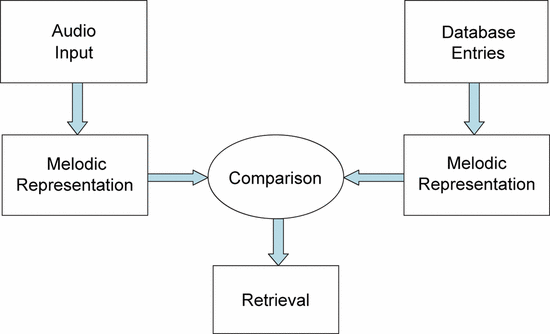
\includegraphics[width=\linewidth]{4432653-fig-1}
        \vspace{-20pt}\caption{Βασικό διάγραμμα ιδέας}
        \label{fig:4432653-fig-1}
\end{wrapfigure}
Η βασική ιδέα του Fingerprinting\cite{fingerapproach2008} παρουσιάζεται στο \imageref{4432653-fig-1}
και συγκεκριμένα ο σιγοτραγουδημένος ήχος και τα στοιχεία της βάσης δεδομένων
πρέπει να αναπαριστώνται με τέτοιο τρόπο, έτσι ώστε να επιτρέπουν ουσιαστικές
συγκρίσεις κατά τη διάρκεια της αναζήτησης και της ανάκτησης. Η είσοδος, λοιπόν,
μεταγράφεται σε μια μελωδική αναπαράσταση στο front-end του συστήματος όπως και
τα περιεχόμενα της βάσης. Οι είσοδοι συγκρίνονται με τα δεδομένα της βάσης και
το σύστημα επιστρέφει το πιο "κατάλληλο" αποτέλεσμα. Παρ' όλα αυτά συχνά
προκύπτει ένας λόγος αβεβαιότητας εξαιτίας της διαφορετικότητας της ερμηνείας
κάθε ατόμου, η οποία προφανώς δεν ταιριάζει πάντα στην αρχική μελωδία στη βάση
δεδομένων. Γι' αυτό ακριβώς προτείνονται μικρά πακέτα υποκείμενης χαρακτηριστικής
πληροφορίας, γνωστά και ως \fps{}, εξαγόμενα από το μουσικό κομμάτι. Έτσι οι
μελωδικές αναπαραστάσεις της εισόδου και της βάσης συγκρίνονται μέσω των
αντίστοιχων \fps{} των κομματιών.

\subsubsection{Προτεινόμενη Προσέγγιση QbSH}
\begin{wrapfigure}{r}{0.5\textwidth}
        \centering
        \vspace{-20pt}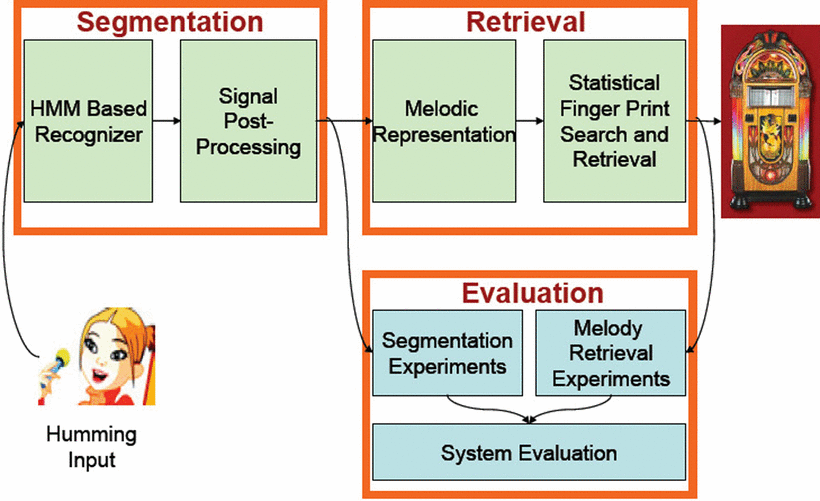
\includegraphics[width=\linewidth]{4432653-fig-2}
        \vspace{-20pt}\caption{Προτεινόμενη προσέγγιση QbSH}
        \label{fig:4432653-fig-2}
\end{wrapfigure}
Για να σχεδιάσουμε ένα εύρωστο σύστημα QbSH, πρέπει να χρησιμοποιήσουμε γνώση
από θεωρία μουσικής καθώς και επεξεργασία σήματος. Έτσι μια προτεινόμενη
προσέγγιση είναι αυτή που παρουσιάζεται στο \imageref{4432653-fig-2}. Ο
σιγοτραγουδημένος ήχος-είσοδος επεξεργάζεται στο πλαίσιο κατάτμησης του
συστήματος χρησιμοποιώντας τεχνικές επεξεργασίας σήματος. Το μέρος ανάκτησης
του συστήματος μετατρέπει πρώτα τον κατακερματισμένο ήχο σε ουσιαστικά μουσικά
σύμβολα βασιζόμενο σε τόνους και διάρκειες, εκμεταλλευόμενο τη μουσική γνώση
και εκτελεί μια εύρωστη αναζήτηση. Το μέρος της αξιολόγησης εξετάζει την
επίδοση των μερών κατακερματισμού του συστήματος καθώς και της ανάκτησης.

\begin{figure}
        \centering
        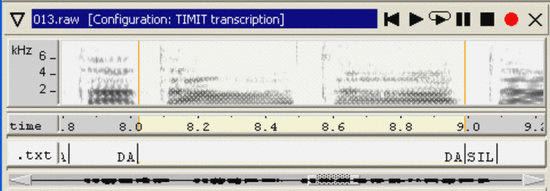
\includegraphics[width=\linewidth]{4432653-fig-6}
        \caption{Σφάλμα διαγραφής στην έξοδο της αναγνώρισης: απουσία ορίου ανάμεσα σε δύο νότες στο κέντρο.}
        \label{fig:4432653-fig-6}
\end{figure}

\subsubsection{Postproccesing}
Ένα πολύ συχνό φαινόμενο είναι αυτό που φαίνεται στο σχήμα \imageref{4432653-fig-6}.
Για να εξαλείψουμε τέτοια φαινόμενα χρησιμοποιούμε ευρετικές μεθόδους βασισμένες στην
πληροφορία ενέργειας και ρυθμού. Εκτός αυτού, χρησιμοποιείται ανάλυση ρυθμού
σαν ένα επιπλέον βήμα για διόρθωση των σφαλμάτων κατακερμάτισης.

\subsubsection{Αναζήτηση και ανάκτηση}
Γίνεται χρήση κυρίως της σχετικής διαφοράς ρυθμού RPD, ο οποίος υπολογίζεται
από το τύπο:
\begin{equation*}
\dfrac{\log(f_k)-\log(f_{k-1})}{\log2^{1/12}}
\end{equation*}
όπου το $f_{k}$ είναι η υπολογισμένη συχνότητα της k-οστής νότας του τραγουδιού
αναζήτησης, καθώς και της σχετικής διαφοράς διάρκειας RDD, η οποία υπολογίζεται
από τον τύπο:

\begin{equation*}
\dfrac{t_k}{t_{k-1}}
\end{equation*}
όπου το $t_{k}$ είναι η διάρκεια της k-οστής νότας.

\subsubsection{Χαρακτηριστικά Fingerprints}
Για να εντοπίσουμε χαρακτηριστικά σημεία στην είσοδο, λαμβάνονται υπόψιν πτυχές
της σύνθεσης μιας μελωδίας. Γίνεται, λοιπόν η υπόθεση ότι οι μεταβολές νότας σε
ένα τόνο μπορούν να θεωρηθούν διακριτικές αν είναι σπάνιες. Για κάθε humming
query, η πιο ευδιάκριτη μετάβαση νότας εντοπίζεται αναζητώντας για την υψηλότερη
αλλαγή επιπέδου βάση RPD και RDD. Τα επιλεγμένα \fps{} πρέπει να περιέχουν αυτά
τα τοπικά χαρακτηριστικά σημεία στον ήχο-είσοδο.

\begin{wrapfigure}[13]{R}{0.5\textwidth}
        \centering
        \vspace{-20pt}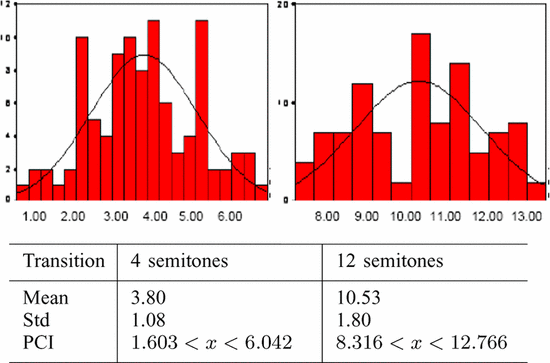
\includegraphics[width=\linewidth]{4432653-fig-10}
        \vspace{-20pt}\caption{Ιστόγραμμα και στατιστικά στοιχεία για δύο μεταβάσεις νότας, κάθε μια εκτελεσμένη 100 φορές.}
        \label{fig:4432653-fig-10}
\end{wrapfigure}

Δεδομένου του μεγάλου εύρους της μουσικής ανάμεσα στα δεδομένα, υπάρχουν υψηλά
επίπεδα αβεβαιότητας και διαφοροποίησης στις λαμβανόμενες εισόδους. Η λύση που
προτείνεται είναι ένα tradeoff, το οποίο είναι βασισμένο σε στατιστικές και
συγκεκριμένα δεδομένα. Για κάθε επίπεδο τόνου και διάρκειας, χτίζεται ένας
δείκτης βεβαιότητας πρόβλεψης κενού το οποίο χρησιμοποιείται όπως το \imageref{4432653-fig-10}.
\undef{\fp}
\undef{\fps}
